% !TEX encoding = UTF-8 Unicode

\chapter{Eigenschaften von \boldmath{$\alpha$}-Shapes}\label{alpha_props}

Da die Menge der $\alpha$-Kreisscheiben einer Punktmenge im Allgemeinen unendlich groß ist, kann sie nicht direkt zur Bestimmung der $\alpha$-Shape verwendet werden.

In diesem Kapitel soll gezeigt werden, dass die $\alpha$-Shape ein Subgraph des Delaunay-Graphen ist. Das Shape-Spektrum ermöglicht die schnelle Identifizierung der Knoten und Kanten der $\alpha$-Shape in den Knoten und Kanten des Delaunay-Graphen. Der Delaunay-Graph und das Shape-Spektrum werden mit Hilfe des \- Voronoi-Diagramms bestimmt.

Für die folgenden Definitionen sei wieder eine Punktmenge $S$ gegeben. Die definierten Begriffe beziehen sich immer auf diese Punktmenge.

\section{Das Voronoi-Diagramm}

Das Voronoi-Diagramm von $S$ ist eine Unterteilung der Ebene in Voronoi-Zellen. Jede Zelle hat ein Zentrum, welches ein Punkt $P \in S$ ist. Ob ein Punkt $P_i$ der Ebene in einer Zelle liegt ist vom Abstand des Punktes $P_i$ zum Zentrum $P$ der Zelle abhängig. Es gibt zwei Ausprägungen des Voronoi-Diagramms. In der ersten Ausprägung ist das Kriterium, ob ein Punkt der Ebene in einer Zelle liegt, ein möglichst kleiner Abstand zu ihrem Zentrum.

\begin{defin}
Das \emph{Voronoi-Diagramm \- der \- Punkte \- mit \- minimalem \- Abstand}, \- $VD_{\min}(S)$, \- ist eine vollständige Unterteilung der Ebene in Teilflächen, den sogenannten Voronoi-Zellen. Für jeden Punkt $P \in S$ existiert eine eindeutige \emph{Voronoi-Zelle der Punkte mit minimalem Abstand} $VC_{\min}(P)$. $P$ ist das Zentrum dieser Zelle. Der Abstand jedes Punktes $P_i \in VC_{\min}(P)$ zu $P$ ist kleiner oder gleich dem Abstand von $P_i$ zu einem anderen Zentrum.
\end{defin}

Das Voronoi-Diagramm der Punkte mit minimalem Abstand wird im Folgenden auch kurz als Minimum-Voronoi-Diagramm und die zugehörige Voronoi-Zelle als Minimum-Voronoi-Zelle bezeichnet.

In der zweiten Ausprägung des Voronoi-Diagramms ist das Kriterium, ob ein Punkt der Ebene zu einer Zelle gehört, ein möglichst großer Abstand zu ihrem Zentrum.

\begin{defin}
Das \emph{Voronoi-Diagramm \- der \- Punkte \- mit \- maximalem \- Abstand}, \- $VD_{\max}(S)$, \- ist eine vollständige Unterteilung der Ebene in Voronoi-Zellen. Für jeden Punkt $P \in S$, welcher auf dem Rand der konvexen Hülle liegt, existiert eine eindeutige \emph{Voronoi-Zelle der Punkte mit maximalem Abstand} $VC_{\max}(P)$. $P$ ist das Zentrum dieser Zelle. Der Abstand jedes Punktes $P_i \in VC_{\max}(P)$ zu $P$ ist größer oder gleich dem Abstand von $P_i$ zu einem anderen Zentrum.
\end{defin}

Das Voronoi-Diagramm der Punkte mit maximalem Abstand wird im Folgenden auch kurz als Maximum-Voronoi-Diagramm und die zugehörige Voronoi-Zelle als Maximum-Voronoi-Zelle bezeichnet.

\begin{figure}[htbp]
	\centering
	\subfloat[Minimum-Voronoi-Diagramm und -Zelle\label{fig:voronoi_min}]
		{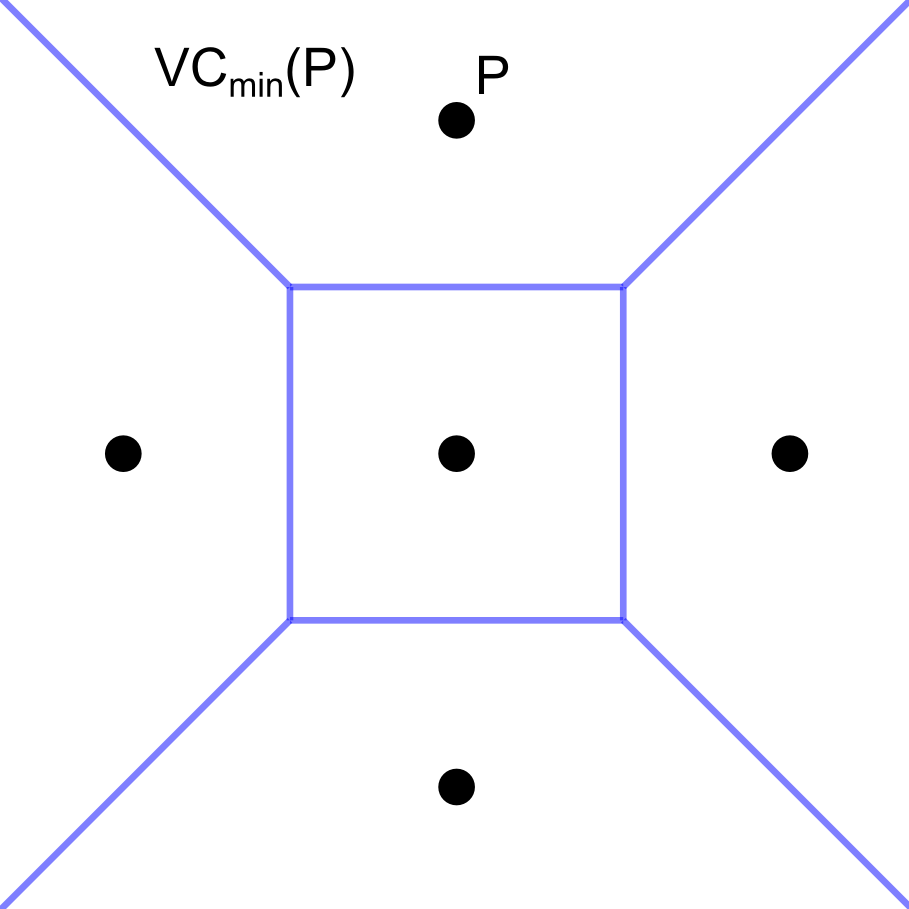
\includegraphics[scale=0.7]{../bilder/voronoi_min.png}}
	\hspace{2cm}
	\subfloat[Maximum-Voronoi-Diagramm und -Zelle\label{fig:voronoi_max}]
		{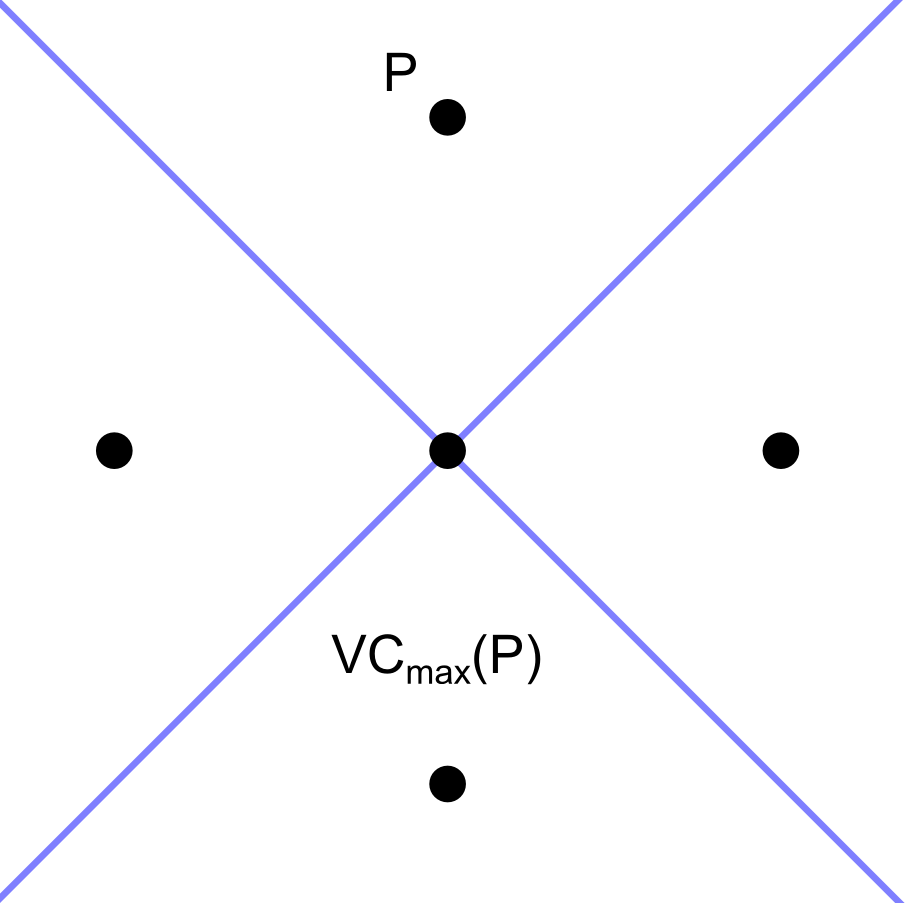
\includegraphics[scale=0.7]{../bilder/voronoi_max.png}}
	\caption{Voronoi-Diagramme und -Zellen}
	\label{fig:voronoi}	
\end{figure}

Abbildung~\ref{fig:voronoi} zeigt das Minimum- und Maximum-Voronoi-Diagramm einer einfachen Punktmenge sowie je eine beschriftete Zelle und ihr Zentrum.

\begin{eigen}
Sei $B$ die Menge der Strecken, Strahlen und Geraden, welche die Voronoi-Zellen eines Voronoi-Diagramms begrenzen. Jedes $b \in B$ liegt auf der Streckenhalbierenden zwischen den Zentren $P_1$ und $P_2$ zweier Voronoi-Zellen und trennt diese voneinander. Der Abstand eines Punktes $P_b \in b$ zu $P_1$ ist daher gleich dem Abstand von $P_b$ zu $P_2$ und $P_b$ liegt in beiden Voronoi-Zellen.
\end{eigen}

Das Voronoi-Diagramm ist eine Einbettung des Voronoi-Graphen in die Ebene. Der Voronoi-Graph kann über das Voronoi-Diagramm definiert werden.

\begin{defin}
Gegeben sei ein Voronoi-Diagramm. Die Strecken, Strahlen und Geraden, welche die Voronoi-Zellen des Voronoi-Diagramms begrenzen, sind die \emph{Kanten des Voronoi-Graphen}. Die Endpunkte der Strecken und die Ursprünge der Strahlen sind die \emph{Knoten des Voronoi-Graphen}. Zusätzlich existiert ein virtueller Knoten im Unendlichen.\\
Die Strecken verbinden ihre Endpunkte. Die Strahlen verbinden ihren Ursprung mit dem virtuellen Knoten. Die Geraden verbinden den virtuellen Knoten mit sich selbst.
\end{defin}

\begin{figure}[htbp]
	\centering
	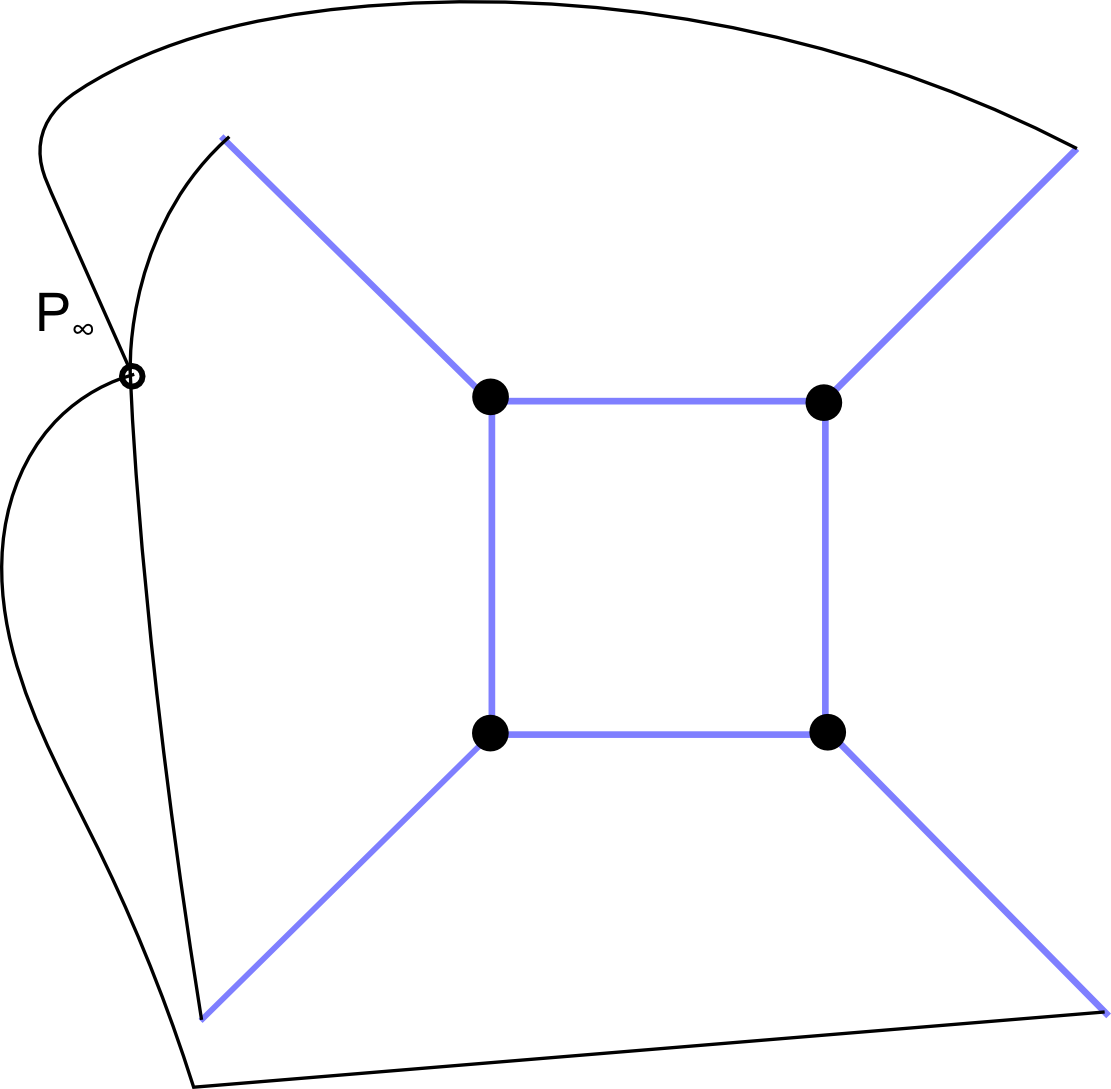
\includegraphics[scale=1.0]{../bilder/voronoiGraph_min.png}
	\caption{Voronoi-Graph mit dem virtuellen Knoten}
	\label{fig:voronoiGraph_min}
\end{figure}

Abbildung~\ref{fig:voronoiGraph_min} zeigt das Minimum-Voronoi-Diagramm aus Abbildung~\ref{fig:voronoi_min} mit dem virtuellen Knoten $P_{\infty}$ und seinen Verbindungen.

\begin{eigen}
Die Kanten des Voronoi-Diagramms kreuzen sich nicht. Damit ist der Voronoi-Graph ein planarer Graph.
\end{eigen}

\section{Der Delaunay-Graph}

Der Delaunay-Graph von $S$ ist ein dualer Graph zum Voronoi-Diagramm von $S$. Für seine Definition wird zuerst definiert, wann zwei Voronoi-Zellen benachbart sind.

\begin{defin}
Gegeben sei ein Voronoi-Diagramm. Zwei \emph{Voronoi-Zellen} sind genau dann \emph{benachbart}, wenn sie eine gemeinsame Kante $b$ besitzen.
\end{defin}

Damit lässt sich der Delaunay-Graph wie folgt definieren.

\begin{defin}
Gegeben sei das Voronoi-Diagramm von $S$. Der \emph{Delaunay-Graph von $S$} ist der Graph, dessen Knoten die Zentren der Voronoi-Zellen sind und dessen Kanten die Zentren benachbarter Voronoi-Zellen verbinden.
\end{defin}

Auch für den Delaunay-Graphen existieren zwei Ausprägungen. Je nachdem aus welchem Voronoi-Diagramm der Graph abgeleitet ist, spricht man vom Delaunay-Graphen der Punkte mit minimalem Abstand, $DG_{\min}(S)$, oder maximalem Abstand, $DG_{\max}(S)$.

Im Folgenden werden auch die Bezeichnungen Minimum-Delaunay-Graph und Maximum-Delaunay-Graph verwendet.

\begin{figure}[htbp]
	\centering
	\subfloat[Minimum-Voronoi-Diagramm und -Delaunay-Graph\label{fig:voronoiDelaunay_min}]
		{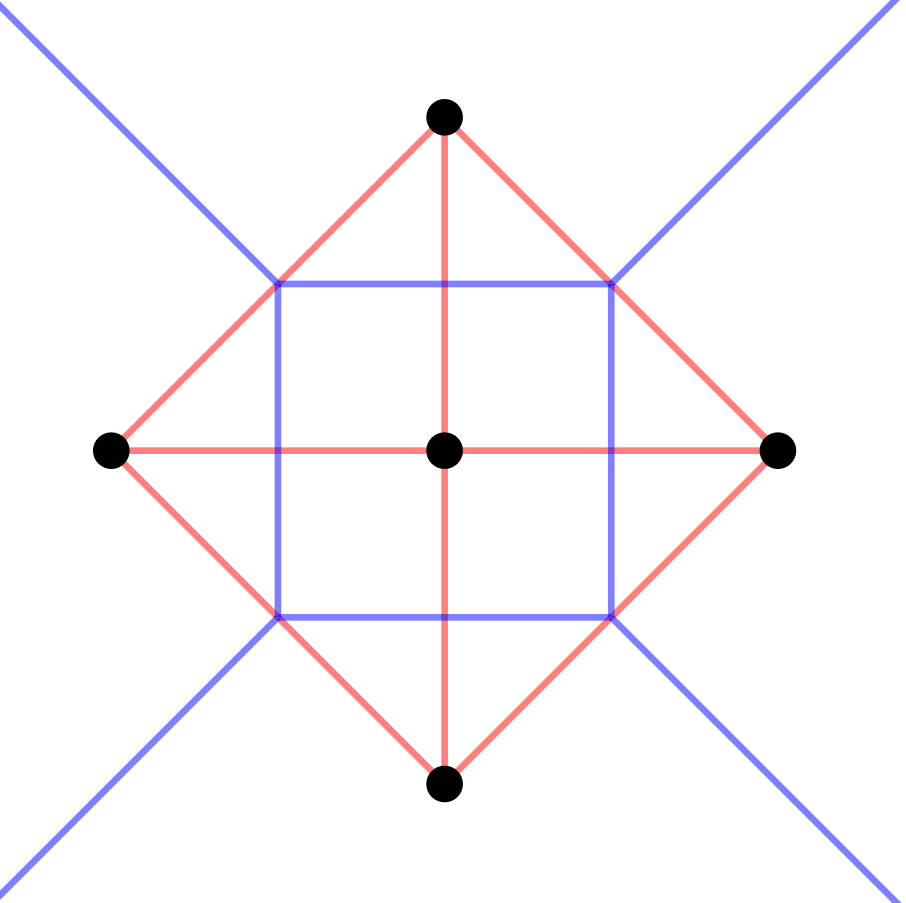
\includegraphics[scale=0.7]{../bilder/voronoiDelaunay_min.png}}
	\hspace{2cm}
	\subfloat[Maximum-Voronoi-Diagramm und -Delaunay-Graph\label{fig:voronoiDelaunay_max}]
		{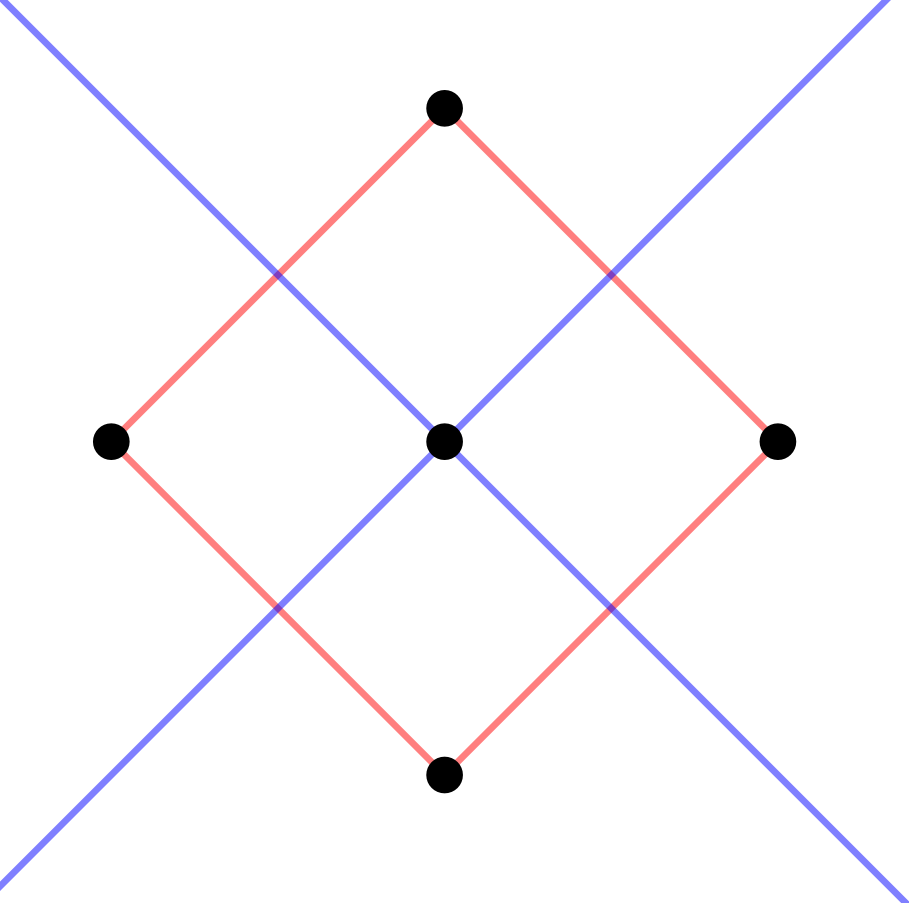
\includegraphics[scale=0.7]{../bilder/voronoiDelaunay_max.png}}
	\caption{Voronoi-Diagramme und Delaunay-Graphen}
	\label{fig:voronoiDelaunay}	
\end{figure}

Abbildung~\ref{fig:voronoiDelaunay} zeigt Minimum- und Maximum-Voronoi-Diagramme sowie die zugehörigen Delaunay-Graphen einer einfachen Punktmenge.

\section[Die $\alpha$-Shape als Subgraph des Delaunay-Graphen]{Die \boldmath{$\alpha$}-Shape als Subgraph des Delaunay-Graphen}

Die $\alpha$-Shape ist ein Subgraph des Delaunay-Graphen. Folgende Eigenschaften des Voronoi-Diagramms und des Delaunay-Graphen sind für den Beweis dafür wichtig. Alle Aussagen gelten sowohl für positve $\alpha$-Shape und -Kreisscheiben in Bezug auf Minimum-Voronoi-Diagramm und -Delaunay-Graph als auch für negative $\alpha$-Shape und -Kreisscheiben in Bezug auf Maximum-Voronoi-Diagramm und -Delaunay-Graph.

\begin{eigen}\label{eigen_alphaExtreme_VD}
Gegeben sei das Voronoi-Diagramm von $S$. Sei eine beliebige Voronoi-Zelle mit einem Zentrum $P \in S$ gegeben. Diese Zelle ist der Ort der Mittelpunkte $P_C$ derjenigen $\alpha$-Kreisscheiben, welche $P$ auf ihrem Rand haben. Der Radius einer solchen $\alpha$-Kreisscheibe ist gleich dem Abstand von $P_C$ zu $P$. Kein anderer Ort kann Mittelpunkt einer solchen $\alpha$-Kreisscheibe sein.
\end{eigen}

\begin{figure}[htbp]
	\centering
	\subfloat[Positive $\alpha$-Kreisscheibe und Minimum-Voronoi-Zelle\label{fig:alphaExtreme_VDmin}]
		{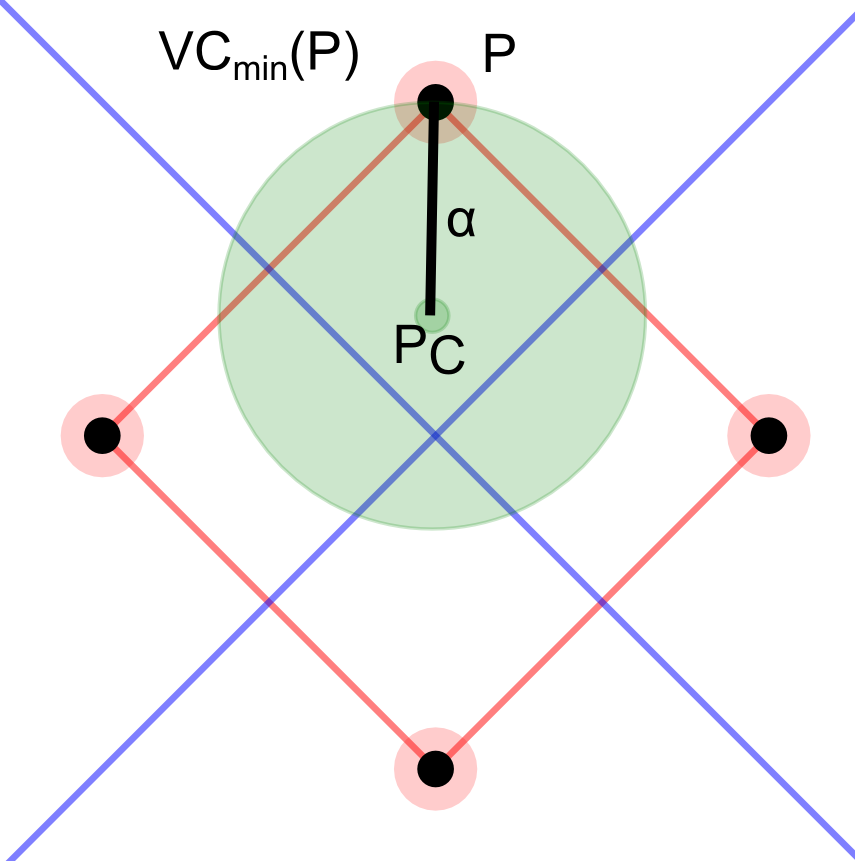
\includegraphics[scale=0.7]{../bilder/alphaExtreme_VDmin.png}}
	\hspace{2cm}
	\subfloat[Negative $\alpha$-Kreisscheibe und Maximum-Voronoi-Zelle\label{fig:alphaExtreme_VDmax}]
		{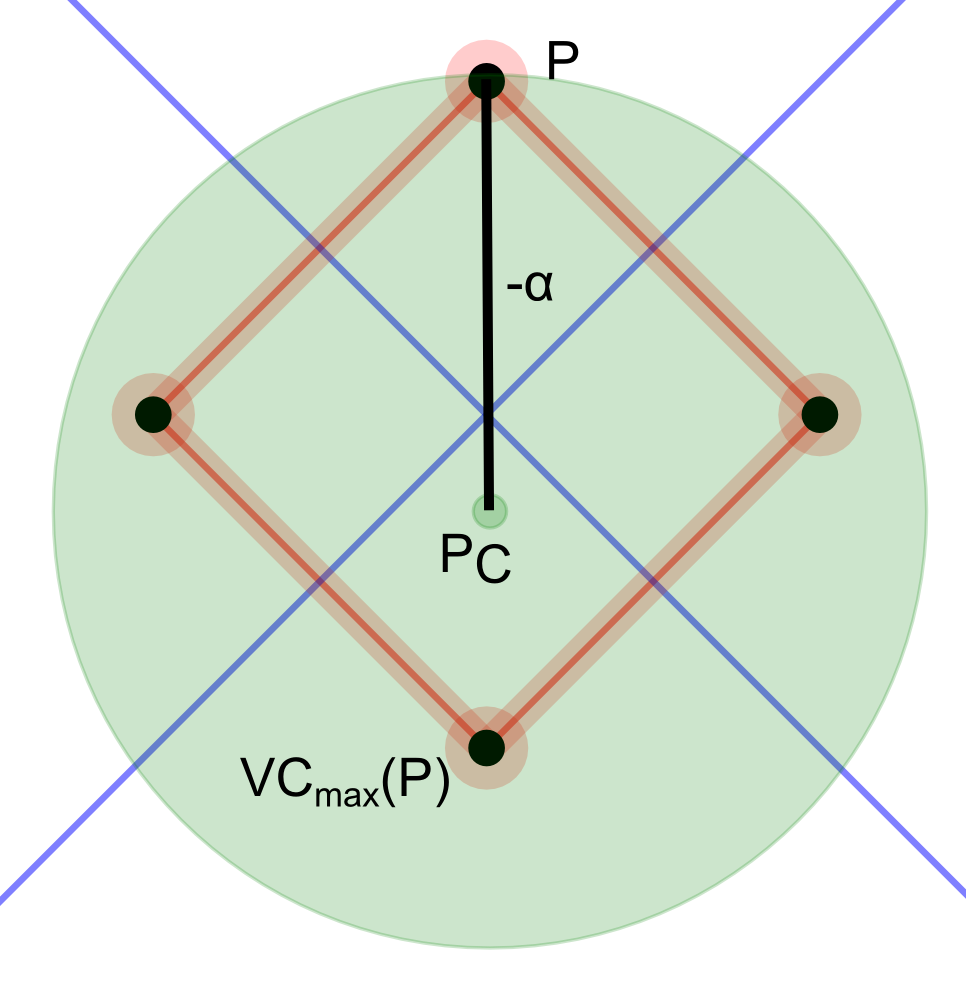
\includegraphics[scale=0.7]{../bilder/alphaExtreme_VDmax.png}}
	\caption{$\alpha$-Kreisscheiben mit Mittelpunkten in Voronoi-Zellen}
	\label{fig:alphaExtreme_VD}	
\end{figure}

Abbildung~\ref{fig:alphaExtreme_VD} stellt Beispiele zu Eigenschaft \ref{eigen_alphaExtreme_VD} dar.

\begin{eigen}\label{eigen_alphaNeighbours_VD}
Gegeben sei das Voronoi-Diagramm von $S$. Sei $b$ die Kante zwischen den Voronoi-Zellen mit den Zentren $P_1,P_2 \in S$. Die Kante $b$ ist der Ort der Mittelpunkte $P_C$ derjenigen $\alpha$-Kreisscheiben, auf deren Rand $P_1$ und $P_2$ direkt benachbart sind. Der Radius einer solchen $\alpha$-Kreisscheibe ist gleich dem Abstand von $P_1$ und $P_2$ zu $P_C$. Kein anderer Ort kann Mittelpunkt einer solchen Kreisscheibe sein.
\end{eigen}

\begin{figure}[htbp]
	\centering
	\subfloat[Positive $\alpha$-Kreisscheibe und Kante zwischen Minimum-Voronoi-Zellen\label{fig:alphaNeighbours_VDmin}]
		{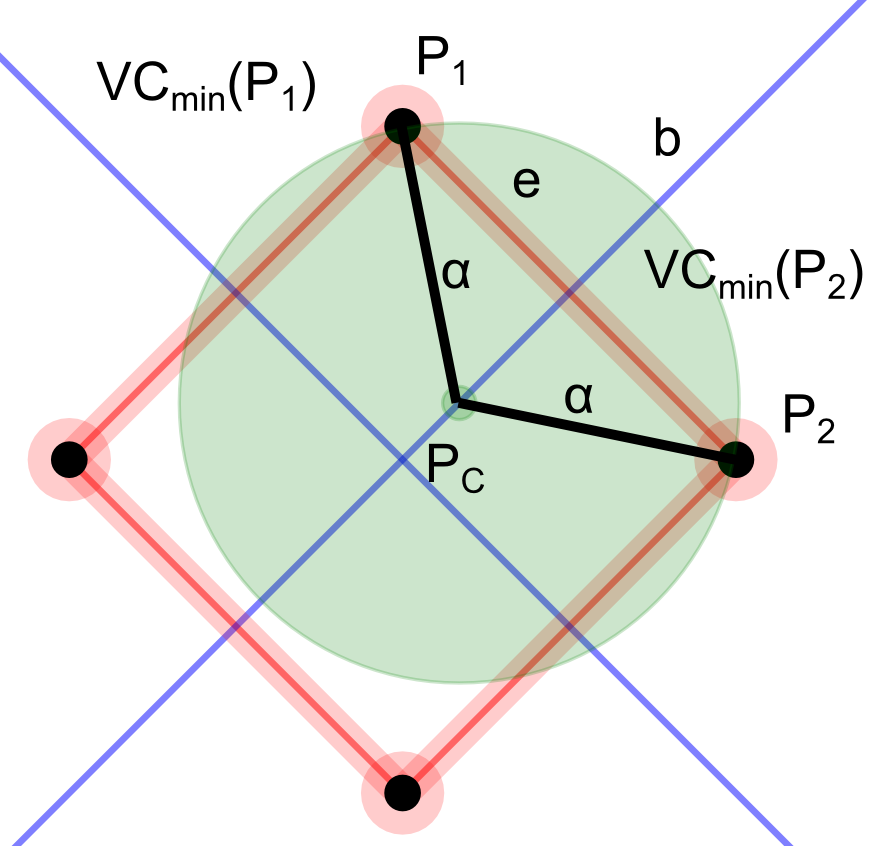
\includegraphics[scale=0.7]{../bilder/alphaNeighbours_VDmin.png}}
	\hspace{2cm}
	\subfloat[Negative $\alpha$-Kreisscheibe und Kante zwischen Maximum-Voronoi-Zellen\label{fig:alphaNeighbours_VDmax}]
		{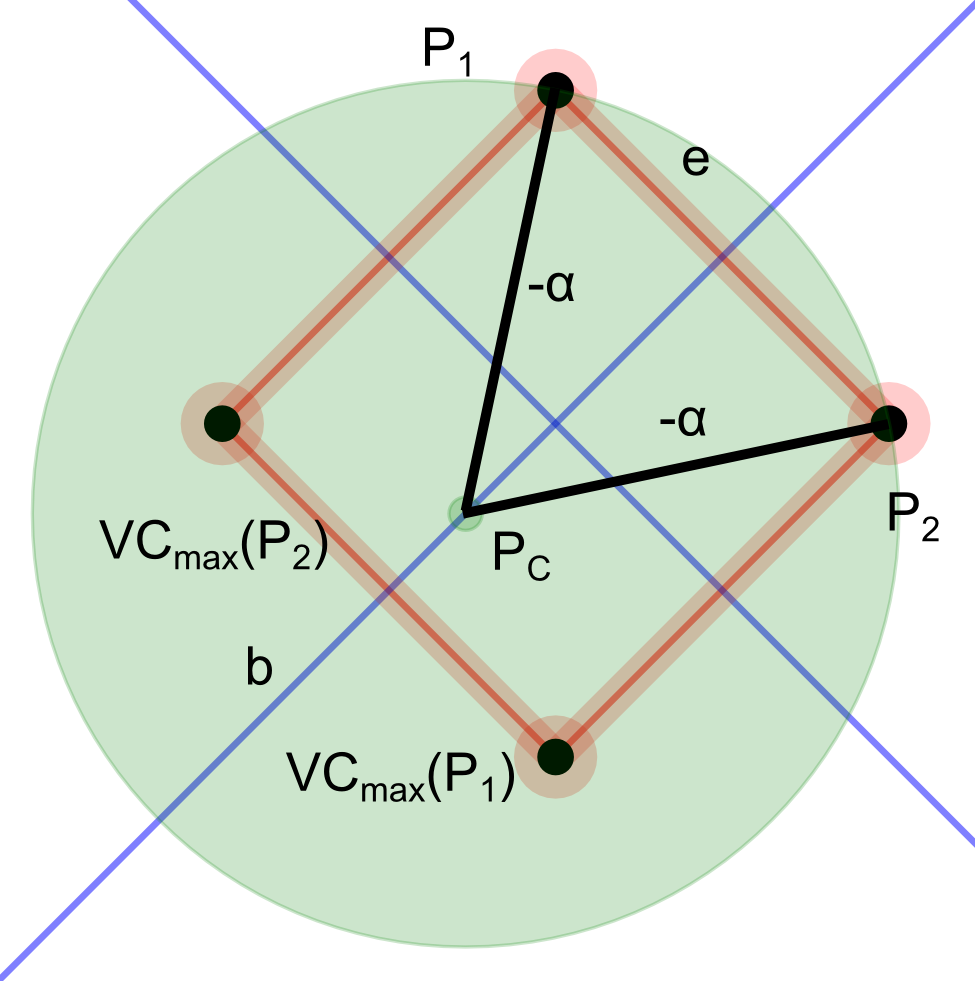
\includegraphics[scale=0.7]{../bilder/alphaNeighbours_VDmax.png}}
	\caption{$\alpha$-Kreisscheiben mit Mittelpunkten auf der gemeinsamen Kante zweier Voronoi-Zellen}
	\label{fig:alphaNeighbours_VD}	
\end{figure}

Abbildung~\ref{fig:alphaNeighbours_VD} stellt Beispiele zu Eigenschaft \ref{eigen_alphaNeighbours_VD} dar.

Hiermit sollen nun folgende Aussagen bewiesen werden.

\begin{lemma}\label{lemma:alphaSubgraph}
Die $\alpha$-Shape von $S$ ist ein Subgraph des Delaunay-Graphen von $S$.
\end{lemma}

Um dies zu Beweisen, wird die Aussage in folgende Teilaussagen zerlegt:

\begin{lemma}\label{lemma:knotenAlphaDelaunay}
Jeder Knoten der $\alpha$-Shape von $S$ ist auch ein Knoten des Delaunay-Graphen von $S$.
\end{lemma}

\begin{proof}[Beweis zu Lemma \ref{lemma:knotenAlphaDelaunay}]
Sei $P \in S$ ein Knoten der $\alpha$-Shape von $S$. Daraus folgt, dass $P$ auf dem Rand mindestens einer $\alpha$-Kreisscheibe liegt. Der einzig mögliche Ort für Mittelpunkte $P_C$ solcher Kreisscheiben ist diejenige Voronoi-Zelle, welche $P$ als Zentrum hat. Da jedes Zentrum einer Voronoi-Zelle einem Knoten im Delaunay-Graphen enstpricht, ist $P$ auch ein Knoten des Delaunay-Graphen von $S$.
\end{proof}

\begin{lemma}\label{lemma:kanteAlphaDelaunay}
Jede Kante der $\alpha$-Shape von $S$ ist auch eine Kante des Delaunay-Graphen von $S$.
\end{lemma}

\begin{proof}[Beweis zu Lemma \ref{lemma:kanteAlphaDelaunay}]
Sei $e$ eine Kante der $\alpha$-Shape von $S$. Daraus folgt, dass $e$ zwei $\alpha$-Nachbarn $P_1,P_2 \in S$ verbindet. $\alpha$-Nachbarn sind auf dem Rand mindestens einer $\alpha$-Kreisscheibe direkt benachbart. Der einzig mögliche Ort für Mittelpunkte $P_C$ solcher Kreisscheiben ist die Voronoi-Kante $b$ zwischen den beiden Voronoi-Zellen, welche $P_1$ und $P_2$ als Zentrum haben. Da mindestens ein $P_C$ existiert muss auch $b$ existieren. Da $b$ existiert, sind die Voronoi-Zellen benachbart und $e$ ist damit auch eine Kante im Delaunay-Graphen von $S$.
\end{proof}

\begin{lemma}\label{lemma:knotenDelaunayAlpha}
Für jeden Knoten des Delaunay-Graphen von $S$ existiert mindestens ein $\alpha$, für welches der Knoten auch ein Knoten der $\alpha$-Shape von $S$ ist.
\end{lemma}

\begin{proof}[Beweis zu Lemma \ref{lemma:knotenDelaunayAlpha}]
Sei $P \in S$ ein Knoten des Delaunay-Graphen von $S$. Daraus folgt, dass $P \in S$ das Zentrum einer Voronoi-Zelle ist. Sei $P_C$ ein Punkt innerhalb dieser Voronoi-Zelle. Sei der Betrag von $\alpha$ gleich dem Abstand von $P_C$ zu $P$. Für ein solches $\alpha$ liegt $P$ auf dem Rand der $\alpha$-Kreisscheibe mit Mittelpunkt $P_C$ und ist somit $\alpha$-extrem. Somit ist $P$ auch ein Knoten der $\alpha$-Shape von $S$.
\end{proof}

\begin{lemma}\label{lemma:kanteDelaunayAlpha}
Für jede Kante des Delaunay-Graphen von $S$ existiert mindestens ein $\alpha$, für welches die Kante auch eine Kante der $\alpha$-Shape von $S$ ist.
\end{lemma}

\begin{proof}[Beweis zu Lemma \ref{lemma:kanteDelaunayAlpha}]
Sei $e$ eine Kante des Delaunay-Graphen von $S$. Die Kante verbindet die Zentren $P_1,P_2 \in S$ zweier benachbarter Voronoi-Zellen. Sei $b$ die Voronoi-Kante zwischen diesen Voronoi-Zellen. Sei $P_C$ ein beliebiger Punkt auf $b$. Der Betrag von $\alpha$ sei gleich dem Abstand von $P_C$ zu $P_1$ und $P_2$. Für ein solches $\alpha$ sind $P_1$ und $P_2$ direkt auf dem Rand der $\alpha$-Kreisscheibe mit Mittelpunkt $P_C$ benachbart und sind somit $\alpha$-Nachbarn. Somit ist $e$ auch eine Kante der $\alpha$-Shape von $S$.
\end{proof}

\begin{proof}[Beweis zu Lemma \ref{lemma:alphaSubgraph}]
Aus der Richtigkeit der Lemmata \ref{lemma:knotenAlphaDelaunay}, \ref{lemma:kanteAlphaDelaunay}, \ref{lemma:knotenDelaunayAlpha} und \ref{lemma:kanteDelaunayAlpha} folgt die Richtigkeit von Lemma \ref{lemma:alphaSubgraph}.
\end{proof}

\section{Das Shape-Spektrum}

Das Shape-Spektrum wird zur Konstruktion einer $\alpha$-Shape aus einem Delaunay-Graphen verwendet werden. Es ist folgendermaßen definiert.

\begin{defin}
Das \emph{positive Shape-Spektrum}, $Sp^+$, \emph{eines Knotens bzw. einer Kante des Minimum-Delaunay-Graphen von $S$} ist die Menge aller positiven $\alpha$, für welche der Knoten bzw. die Kante ein Teil der $\alpha$-Shape von $S$ ist.
Das \emph{negative Shape-Spektrum}, $Sp^-$, \emph{eines Knotens bzw. einer Kante eines Maximum-Delaunay-Graphen von $S$} ist die Menge aller negativen $\alpha$, für welche der Knoten bzw. die Kante ein Teil der $\alpha$-Shape von $S$ ist.
\end{defin}

Folgende Eigenschaften des Voronoi-Diagramms können für die Bestimmung der Shape-Spektren verwendet werden.

\begin{eigen}
Die Zentren der Zellen des Minimum-Voronoi-Diagramms von $S$ liegen innerhalb ihrer Zellen. Die Zentren der Zellen des Maximum-Voronoi-Diagramms von $S$ liegen, für $\mid S \mid > 1$, außerhalb ihrer Zellen. Für $\mid S \mid = 1$ besteht das Voronoi-Diagramm genau aus einer Zelle, welche die gesamte Ebene einnimmt. Das Zentrum dieser Zelle liegt in der Ebene und damit auch in der Zelle. 
\end{eigen}

\begin{eigen}
Sei ein Voronoi-Diagramm von $S$ gegeben. Sei $P \in S$ ein Punkt, welcher nicht auf dem Rand der konvexen Hülle von $S$ liegt. Die Voronoi-Zelle mit dem Zentrum $P$ ist eine endliche Teilfläche der Ebene.
\end{eigen}

\begin{eigen}
Sei ein Voronoi-Diagramm von $S$ gegeben. Sei $P \in S$ ein Punkt, welcher auf dem Rand der konvexen Hülle von $S$ liegt. Die Voronoi-Zelle mit dem Zentrum $P$ ist eine unendliche Teilfläche der Ebene.
\end{eigen}

\begin{eigen}
Sei ein Voronoi-Diagramm von $S$ gegeben. Seien $P_1,P_2 \in S$ zwei Punkte, welche nicht direkt auf dem Rand der konvexen Hülle von $S$ benachbart sind. Die Kante zwischen den Voronoi-Zellen mit den Zentren $P_1$ und $P_2$ ist eine Strecke.
\end{eigen}

\begin{eigen}
Sei ein Voronoi-Diagramm von $S$ gegeben. Seien $P_1,P_2 \in S$ zwei Punkte, welche direkt auf dem Rand der konvexen Hülle von $S$ benachbart sind. Die Kante zwischen den Voronoi-Zellen mit den Zentren $P_1$ und $P_2$ ist ein Strahl oder eine Gerade.
\end{eigen}

Mit diesen Eigenschaften lassen sich die Shape-Spektren bestimmen.

\begin{lemma}\label{lemma:alphaExtreme_VDmin_alphaMax}
Sei $P \in S$ ein Knoten des Minimum-Delaunay-Graphen von $S$, welcher nicht auf dem Rand der konvexen Hülle von $S$ liegt. Dann gilt $Sp^+(P) = (0, \alpha_{\max}]$. $\alpha_{\max}$ ist der maximale Abstand von $P$ zum Rand seiner Voronoi-Zelle. 
\end{lemma}

\begin{figure}[htbp]
	\centering
	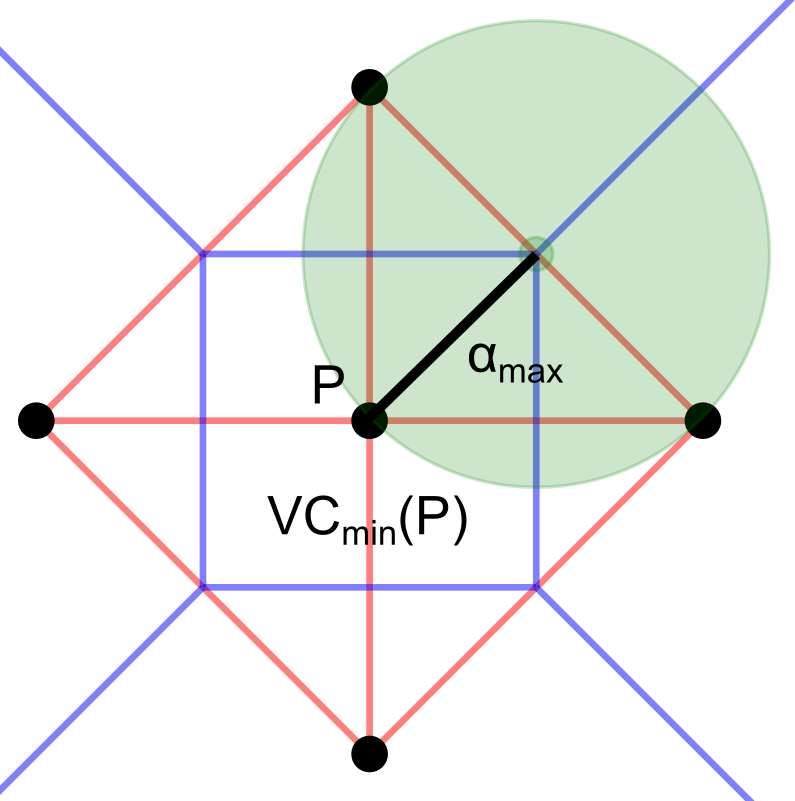
\includegraphics[scale=0.7]{../bilder/alphaExtreme_VDmin_alphaMax.png}
	\caption{$\alpha_{\max}$ für einen Knoten $P$ aus $DG_{\min}$, welcher nicht auf dem Rand der konvexen Hülle liegt}
	\label{fig:alphaExtreme_VDmin_alphaMax}
\end{figure}

Abbildung~\ref{fig:alphaExtreme_VDmin_alphaMax} zeigt ein Beispiel für die in Lemma \ref{lemma:alphaExtreme_VDmin_alphaMax} geschilderte Situation.

\begin{proof}[Beweis zu Lemma \ref{lemma:alphaExtreme_VDmin_alphaMax}]
Sei das Minimum-Voronoi-Diagramm von $S$ gegeben. Die Voronoi-Zelle mit Zentrum $P \in S$ ist der einzige Ort für Mittelpunkte von positiven $\alpha$-Kreisscheiben, welche $P$ auf ihrem Rand haben. Der Radius einer solchen $\alpha$-Kreisscheibe kann beliebig klein sein, da $P$ in seiner Voronoi-Zelle liegt. Der Radius ist nach oben begrenzt, da die Voronoi-Zellen von Punkten, welche nicht auf dem Rand der konvexen Hülle liegen, endliche Teilflächen der Ebene sind.
\end{proof}

\begin{lemma}\label{lemma:alphaExtreme_VDmin_Konvex}
Sei $P \in S$ ein Knoten des Minimum-Delaunay-Graphen von $S$, welcher auf dem Rand der konvexen Hülle von $S$ liegt. Dann gilt $Sp^+(P) = (0, \infty)$.
\end{lemma}

\begin{figure}[htbp]
	\centering
	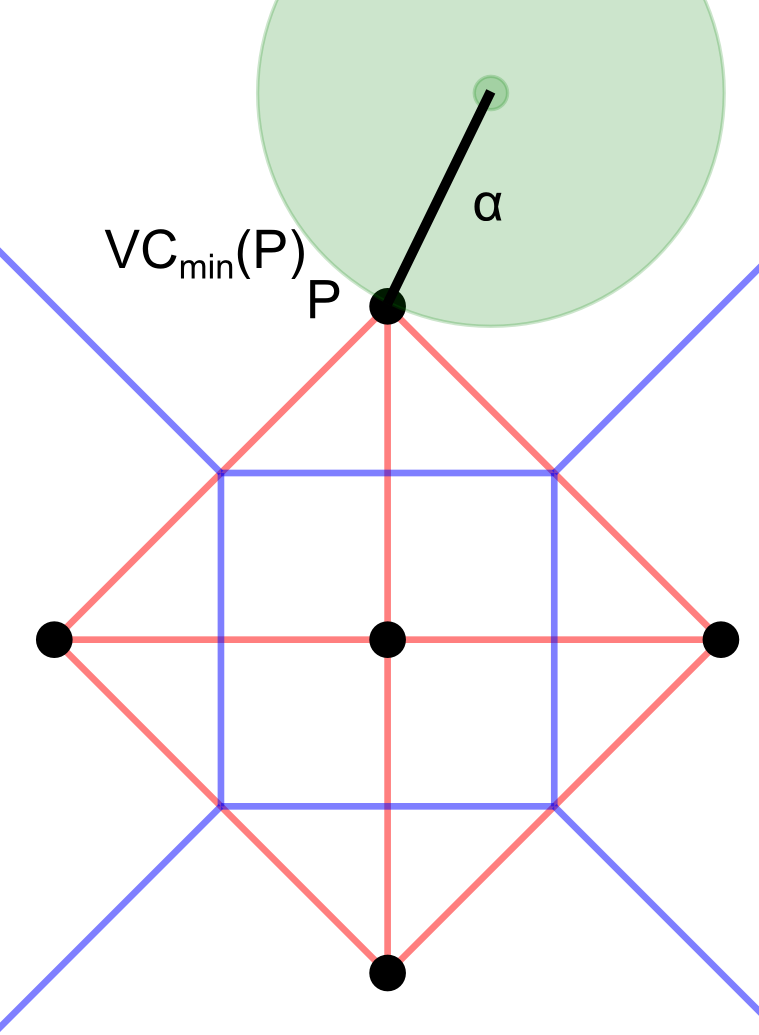
\includegraphics[scale=0.7]{../bilder/alphaExtreme_VDmin_Konvex.png}
	\caption{Beliebiges $\alpha$ für einen Knoten $P$ aus $DG_{\min}$, welcher auf dem Rand der konvexen Hülle liegt}
	\label{fig:alphaExtreme_VDmin_Konvex}
\end{figure}

Abbildung~\ref{fig:alphaExtreme_VDmin_Konvex} zeigt ein Beispiel für die in Lemma \ref{lemma:alphaExtreme_VDmin_Konvex} geschilderte Situation.

\begin{proof}[Beweis zu Lemma \ref{lemma:alphaExtreme_VDmin_Konvex}]
Sei das Minimum-Voronoi-Diagramm von $S$ gegeben. Die Voronoi-Zelle mit Zentrum $P \in S$ ist der einzige Ort für Mittelpunkte von positiven $\alpha$-Kreisscheiben, welche $P$ auf ihrem Rand haben. Der Radius einer solchen $\alpha$-Kreisscheibe kann beliebig klein sein, da $P$ in seiner Voronoi-Zelle liegt. Der Radius ist nicht nach oben begrenzt, da die Voronoi-Zellen von Punkten, welche auf dem Rand der konvexen Hülle liegen, unendliche Teilflächen der Ebene sind.
\end{proof}

\begin{lemma}\label{lemma:alphaExtreme_VDmax_alphaMax}
Sei $P \in S$ ein Knoten des Maximum-Delaunay-Graphen von $S$. Dann gilt $Sp^-(P) = (-\infty, \alpha_{\max}]$. $\alpha_{\max}$ ist die Negation des minimalen Abstands von $P$ zum Rand seiner Voronoi-Zelle. 
\end{lemma}

\begin{figure}[htbp]
	\centering
	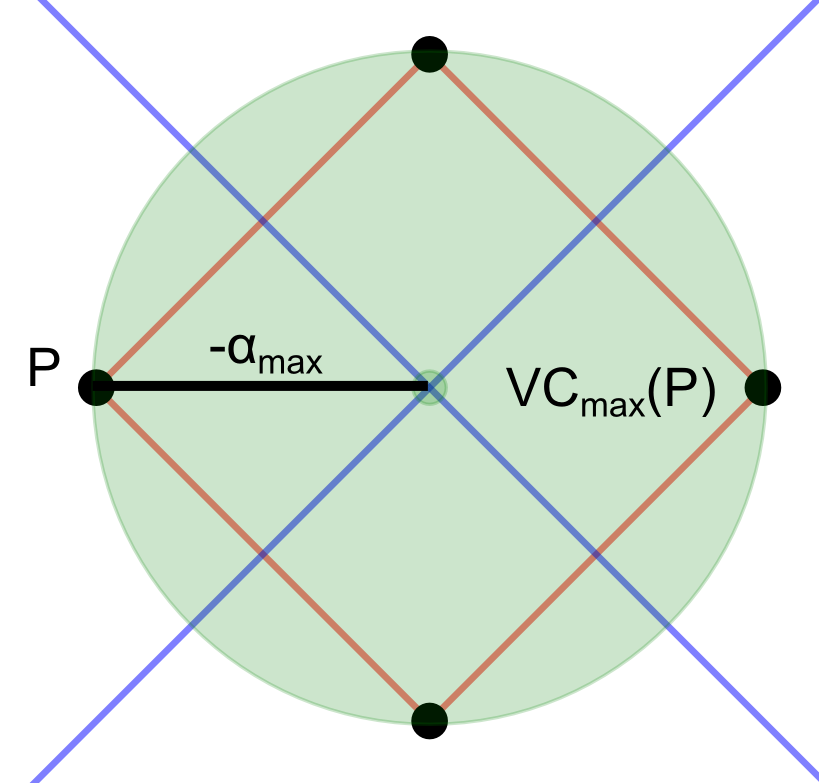
\includegraphics[scale=0.7]{../bilder/alphaExtreme_VDmax_alphaMax.png}
	\caption{$\alpha_{\max}$ für einen Knoten $P$ aus $DG_{\max}$}
	\label{fig:alphaExtreme_VDmax_alphaMax}
\end{figure}

Abbildung~\ref{fig:alphaExtreme_VDmax_alphaMax} zeigt ein Beispiel für die in Lemma \ref{lemma:alphaExtreme_VDmax_alphaMax} geschilderte Situation.

\begin{proof}[Beweis zu Lemma \ref{lemma:alphaExtreme_VDmax_alphaMax}]
Sei das Maximum-Voronoi-Diagramm von $S$ gegeben. Die Voronoi-Zelle mit Zentrum $P \in S$ ist der einzige Ort für Mittelpunkte von negativen $\alpha$-Kreisscheiben, welche $P$ auf ihrem Rand haben. Der Radius einer solchen $\alpha$-Kreisscheibe muss mindestens gleich dem minimalen Abstand von $P$ zu seiner Voronoi-Zelle sein, da $P$ nicht in seiner Voronoi-Zelle liegt. Der Radius ist nicht nach oben begrenzt, da Maximum-Voronoi-Zellen unendliche Teilflächen der Ebene sind, weil ihre Zentren immer auf dem Rand der konvexen Hülle liegen.
\end{proof}

\begin{lemma}\label{lemma:alphaNeighbours_VDmin_alphaMinMax}
Sei $e=(P_1,P_2)$ eine Kante des Minimum-Delaunay-Graphen von $S$. Seien $P_1,P_2 \in S$ nicht direkt auf dem Rand der konvexen Hülle von $S$ benachbart. Sei $b$ die Voronoi-Kante zwischen den Voronoi-Zellen mit den Zentren $P_1$ und $P_2$. Dann gilt $Sp^+(e) = [\alpha_{\min}, \alpha_{\max}]$. $\alpha_{\min}$ ist der minimale und $\alpha_{\max}$ der maximale Abstand von $P_1$ und $P_2$ zu $b$.
\end{lemma}

\begin{figure}[htbp]
	\centering
	\subfloat[$\alpha_{\min}$ für Kante $e$ aus $DG_{\min}$, deren Knoten nicht auf dem Rand der konvexen Hülle benachbart sind\label{fig:alphaNeighbours_VDmin_alphaMin}]
		{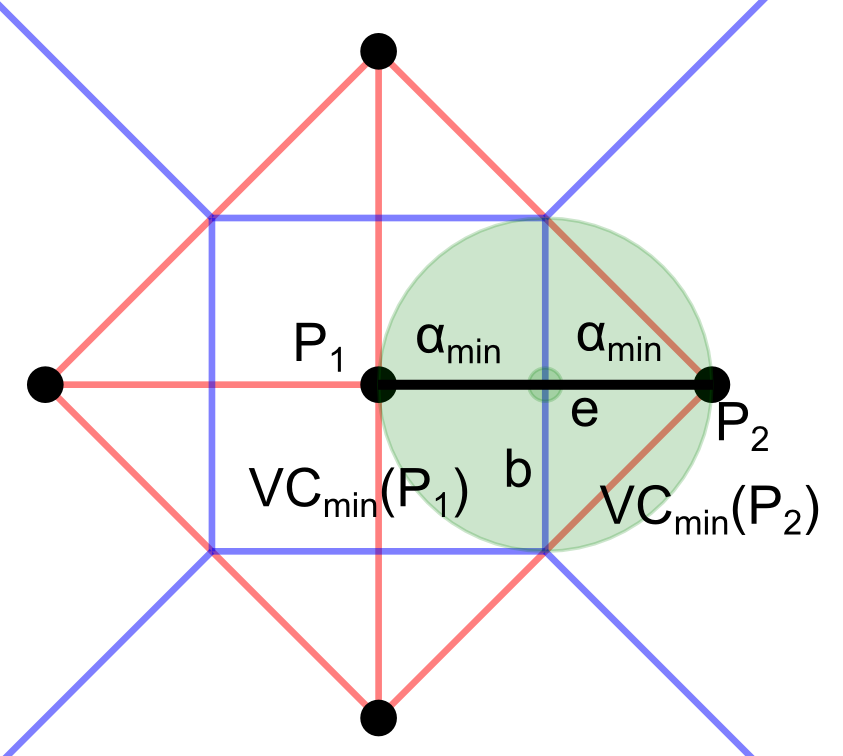
\includegraphics[scale=0.7]{../bilder/alphaNeighbours_VDmin_alphaMin.png}}
	\hspace{2cm}
	\subfloat[$\alpha_{\max}$ für Kante $e$ aus $DG_{\min}$, deren Knoten nicht auf dem Rand der konvexen Hülle benachbart sind\label{fig:alphaNeighbours_VDmin_alphaMax}]
		{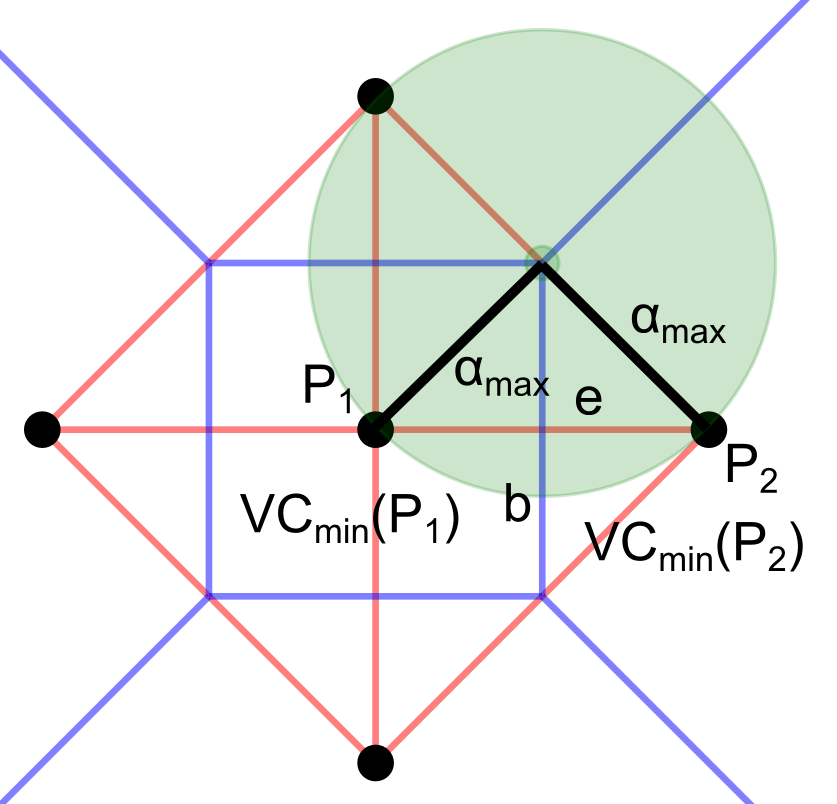
\includegraphics[scale=0.7]{../bilder/alphaNeighbours_VDmin_alphaMax.png}}
	\caption{$\alpha_{\min}$ und $\alpha_{\max}$ für eine Kante $e$ aus $DG_{\min}$, deren Knoten nicht auf dem Rand der konvexen Hülle benachbart sind}
	\label{fig:alphaNeighbours_VDmin_alphaMinMax}	
\end{figure}

Abbildung~\ref{fig:alphaNeighbours_VDmin_alphaMinMax} zeigt Beispiele für die in Lemma \ref{lemma:alphaNeighbours_VDmin_alphaMinMax} geschilderte Situation.

\begin{proof}[Beweis zu Lemma \ref{lemma:alphaNeighbours_VDmin_alphaMinMax}]
Sei das Minimum-Voronoi-Diagramm von $S$ gegeben. Die Voronoi-Kante $b$ zwischen den Voronoi-Zellen mit den Zentren $P_1,P_2 \in S$ ist der einzige Ort für Mittelpunkte von positiven $\alpha$-Kreisscheiben, auf deren Rand $P_1$ und $P_2$ direkt benachbart sind. Der Radius einer solchen $\alpha$-Kreisscheibe muss mindestens gleich dem kleinsten Abstand von $P_1$ und $P_2$ zu $b$ sein. Der Radius kann höchstens gleich dem größten Abstand von $P_1$ und $P_2$ zu $b$ sein.
\end{proof}

\begin{lemma}\label{lemma:alphaNeighbours_VDmin_Konvex}
Sei $e=(P_1,P_2)$ eine Kante des Minimum-Delaunay-Graphen von $S$. Seien $P_1,P_2 \in S$ direkt auf dem Rand der konvexen Hülle von $S$ benachbart. Sei $b$ die Voronoi-Kante zwischen den Voronoi-Zellen mit den Zentren $P_1$ und $P_2$. Dann gilt $Sp^+(e) = [\alpha_{\min}, \infty)$. $\alpha_{\min}$ ist der minimale Abstand von $P_1$ und $P_2$ zu $b$.
\end{lemma}

\begin{figure}[htbp]
	\centering
	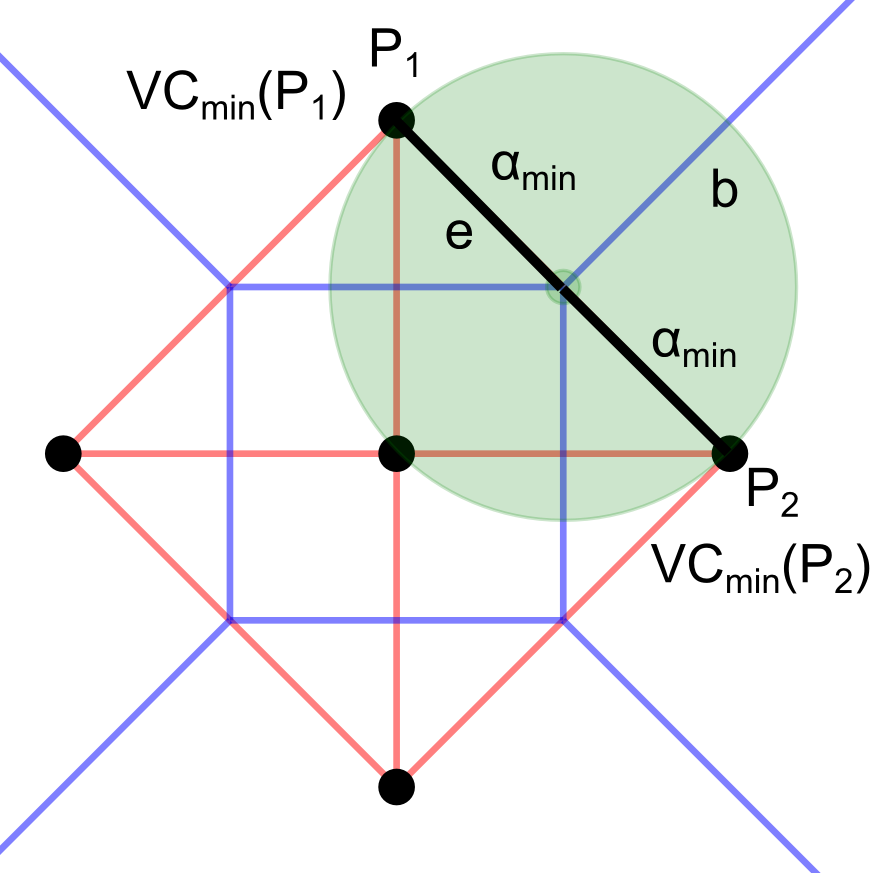
\includegraphics[scale=0.7]{../bilder/alphaNeighbours_VDmin_Konvex.png}
	\caption{$\alpha_{\min}$ für eine Kante $e$ aus $DG_{\min}$, deren Knoten direkt auf dem Rand der konvexen Hülle benachbart sind}
	\label{fig:alphaNeighbours_VDmin_Konvex}
\end{figure}

Abbildung~\ref{fig:alphaNeighbours_VDmin_Konvex} zeigt Beispiele für die in Lemma \ref{lemma:alphaNeighbours_VDmin_Konvex} geschilderte Situation.

\begin{proof}[Beweis zu Lemma \ref{lemma:alphaNeighbours_VDmin_Konvex}]
Sei das Minimum-Voronoi-Diagramm von $S$ gegeben. Die Voronoi-Kante $b$ zwischen den Voronoi-Zellen mit den Zentren $P_1,P_2 \in S$ ist der einzige Ort für Mittelpunkte von positiven $\alpha$-Kreisscheiben, auf deren Rand $P_1$ und $P_2$ direkt benachbart sind. Der Radius einer solchen $\alpha$-Kreisscheibe muss mindestens gleich dem kleinsten Abstand von $P_1$ und $P_2$ zu $b$ sein. Der Radius ist nicht nach oben beschränkt, da $b$ in dem in Lemma \ref{lemma:alphaNeighbours_VDmin_Konvex} geschilderten Fall ein Strahl ist.
\end{proof}

\begin{lemma}\label{lemma:alphaNeighbours_VDmax_alphaMinMax}
Sei $e=(P_1,P_2)$ eine Kante des Maximum-Delaunay-Graphen von $S$. Seien $P_1,P_2 \in S$ nicht direkt auf dem Rand der konvexen Hülle von $S$ benachbart. Sei $b$ die Voronoi-Kante zwischen den Voronoi-Zellen mit den Zentren $P_1$ und $P_2$. Dann gilt $Sp^-(e) = [\alpha_{\min}, \alpha_{\max}]$. $\alpha_{\min}$ ist die Negation des maximalen und $\alpha_{\max}$ die Negation des minimalen Abstands von $P_1$ und $P_2$ zu $b$.
\end{lemma}

\begin{figure}[htbp]
	\centering
	\subfloat[$\alpha_{\min}$ für Kante $e$ aus $DG_{\max}$ deren Knoten nicht auf dem Rand der konvexen Hülle benachbart sind\label{fig:alphaNeighbours_VDmax_alphaMin}]
		{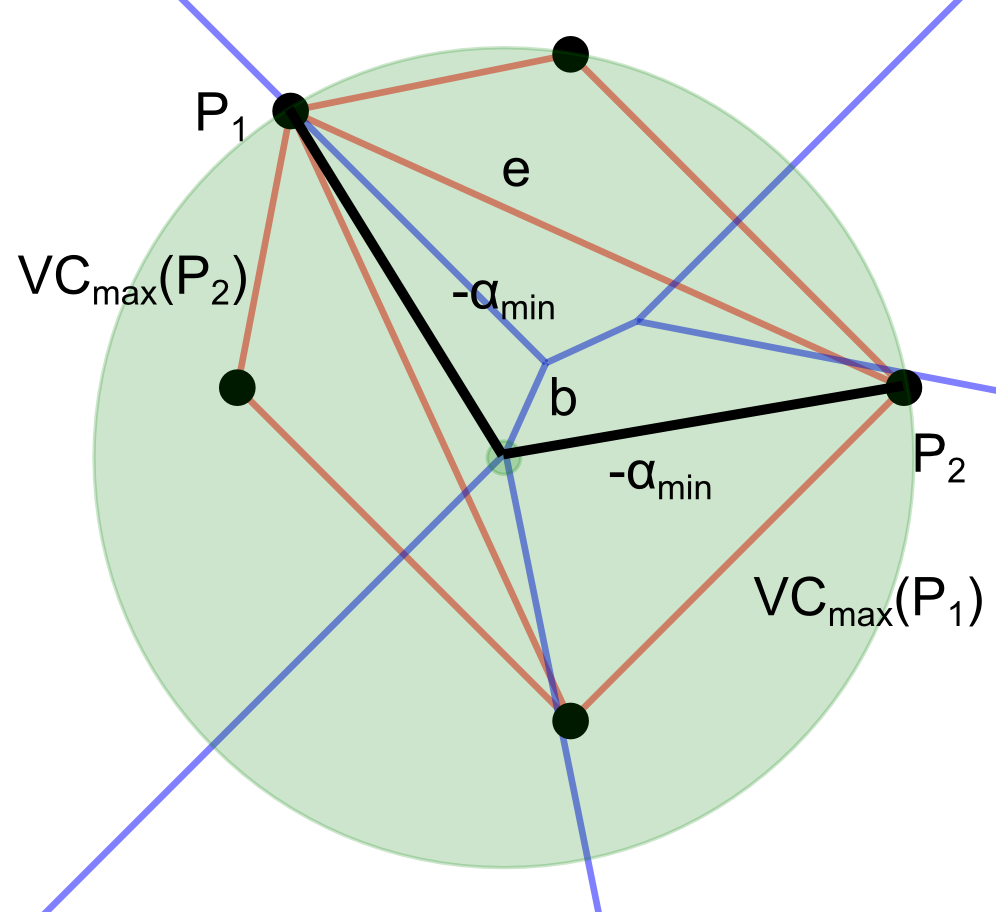
\includegraphics[scale=0.7]{../bilder/alphaNeighbours_VDmax_alphaMin.png}}
	\hspace{2cm}
	\subfloat[$\alpha_{\max}$ für Kante $e$ aus $DG_{\max}$ deren Knoten nicht auf dem Rand der konvexen Hülle benachbart sind\label{fig:alphaNeighbours_VDmax_alphaMax}]
		{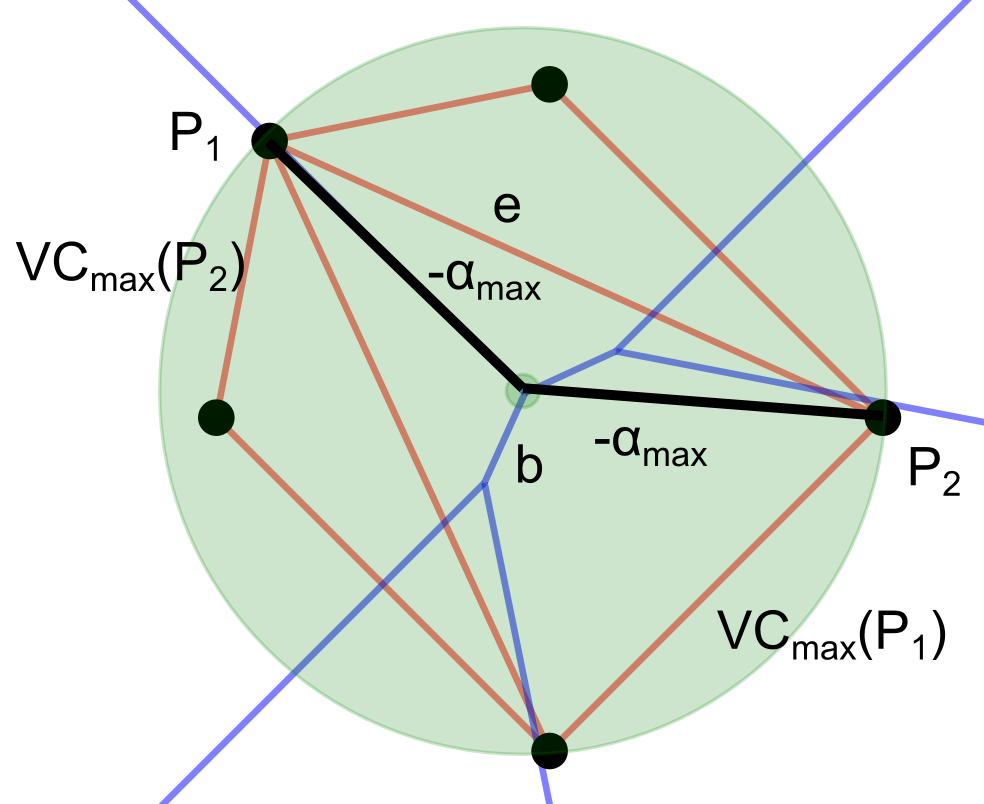
\includegraphics[scale=0.7]{../bilder/alphaNeighbours_VDmax_alphaMax.png}}
	\caption{$\alpha_{\min}$ und $\alpha_{\max}$ für eine Kante $e$ aus $DG_{\max}$ deren Knoten nicht auf dem Rand der konvexen Hülle benachbart sind}
	\label{fig:alphaNeighbours_VDmax_alphaMinMax}	
\end{figure}

Abbildung~\ref{fig:alphaNeighbours_VDmax_alphaMinMax} zeigt Beispiele für die in Lemma \ref{lemma:alphaNeighbours_VDmax_alphaMinMax} geschilderte Situation.

\begin{proof}[Beweis zu Lemma \ref{lemma:alphaNeighbours_VDmax_alphaMinMax}]
Sei das Maximum-Voronoi-Diagramm von $S$ gegeben. Die Voronoi-Kante $b$ zwischen den Voronoi-Zellen mit den Zentren $P_1,P_2 \in S$ ist der einzige Ort für Mittelpunkte von negativen $\alpha$-Kreisscheiben, auf deren Rand $P_1$ und $P_2$ direkt benachbart sind. Der Radius einer solchen $\alpha$-Kreisscheibe muss mindestens gleich dem kleinsten Abstand von $P_1$ und $P_2$ zu $b$ sein. Der Radius kann höchstens gleich dem größten Abstand von $P_1$ und $P_2$ zu $b$ sein.
\end{proof}

\begin{lemma}\label{lemma:alphaNeighbours_VDmax_Konvex}
Sei $e=(P_1,P_2)$ eine Kante des Maximum-Delaunay-Graphen von $S$. Seien $P_1,P_2 \in S$ direkt auf dem Rand der konvexen Hülle von $S$ benachbart. Sei $b$ die Voronoi-Kante zwischen den Voronoi-Zellen mit den Zentren $P_1$ und $P_2$. Dann gilt $Sp^-(e) = (-\infty, \alpha_{\max}]$. $\alpha_{\max}$ ist die Negation des minimale Abstands von $P_1$ und $P_2$ zu $b$.
\end{lemma}

\begin{figure}[htbp]
	\centering
	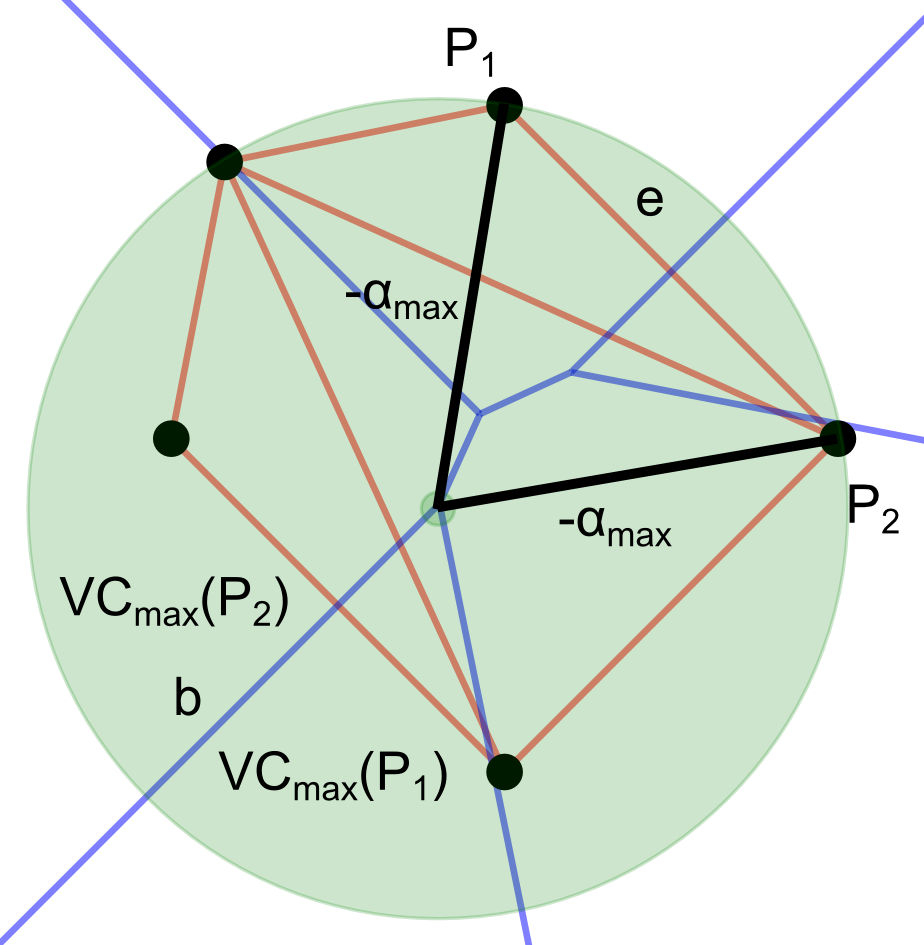
\includegraphics[scale=0.7]{../bilder/alphaNeighbours_VDmax_Konvex.png}
	\caption{$\alpha_{\max}$ für eine Kante $e$ aus $DG_{\max}$ deren Knoten direkt auf dem Rand der konvexen Hülle benachbart sind}
	\label{fig:alphaNeighbours_VDmax_Konvex}
\end{figure}

Abbildung~\ref{fig:alphaNeighbours_VDmax_Konvex} zeigt Beispiele für die in Lemma \ref{lemma:alphaNeighbours_VDmax_Konvex} geschilderte Situation.

\begin{proof}[Beweis zu Lemma \ref{lemma:alphaNeighbours_VDmax_Konvex}]
Sei das Maximum-Voronoi-Diagramm von $S$ gegeben. Die Voronoi-Kante $b$ zwischen den Voronoi-Zellen mit den Zentren $P_1,P_2 \in S$ ist der einzige Ort für Mittelpunkte von negativen $\alpha$-Kreisscheiben, auf deren Rand $P_1$ und $P_2$ direkt benachbart sind. Der Radius einer solchen $\alpha$-Kreisscheibe muss mindestens gleich dem kleinsten Abstand von $P_1$ und $P_2$ zu $b$ sein. Der Radius ist nicht nach oben beschränkt, da $b$ in dem in Lemma \ref{lemma:alphaNeighbours_VDmax_Konvex} geschilderten Fall ein Strahl ist.
\end{proof}

In Lemma \ref{lemma:alphaExtreme_VDmin_alphaMax} - \ref{lemma:alphaNeighbours_VDmax_Konvex} wurde gezeigt, dass die Shape-Spektren von Knoten und Kanten des Delaunay-Graphen Intervalle sind.

Eine Shape-Schwelle ist eine Schwelle, bei deren Überschreiten sich die $\alpha$-Shape ändert. Mit den Shape-Spektren können die Shape-Schwellen einer Punktmenge wie folgt definiert werden.

\begin{defin}
Die Menge der \emph{Shape-Schwellen einer Punktmenge $S$, $Bd(S)$}, ist die Menge der endlichen Grenzen ungleich Null der positiven und negativen Shape-Spektren aller Knoten und Kanten des Minimum- und Maximum-Delaunay-Graphen von $S$.
\end{defin}
